%%%%%%%%%%%%%%%%%%%%%%%%%%%%%%%%%%%%%%%%%%%%%%%%%%%%%%%%%%%%%%%%%%%%%%
% How to use writeLaTeX: 
%
% You edit the source code here on the left, and the preview on the
% right shows you the result within a few seconds.
%
% Bookmark this page and share the URL with your co-authors. They can
% edit at the same time!
%
% You can upload figures, bibliographies, custom classes and
% styles using the files menu.
%
%%%%%%%%%%%%%%%%%%%%%%%%%%%%%%%%%%%%%%%%%%%%%%%%%%%%%%%%%%%%%%%%%%%%%%


 % paper de ref: https://arxiv.org/abs/2204.09082
 
\documentclass[12pt]{article}

\usepackage{sbc-template}

\usepackage{graphicx,url}

%\usepackage[brazil]{babel}   
\usepackage[utf8]{inputenc}  

     
\sloppy

\title{Compiladores e processamento de linguagem natural em SADC}

\author{Fernanda Vitória Nascimento Lisboa\inst{1}, Maria Antônia Amado Lima\inst{1}, Osvaldo Requião Melo\inst{2} }


\address{Centro Universitário SENAI CIMATEC \\
  Caixa Postal 41.650-010 -- Salvador -- BA -- Brasil
\nextinstitute
  Engenharia de Computação -- Centro Universitário SENAI CIMATEC  \\
  Salvador, Brasil
  \email{\{fernanda.lisboa,maria.lima\}@aln.senaicimatec.edu.br
  }
  \email{osvaldo.melo@doc.senaicimatec.edu.br}
}

\begin{document} 

\maketitle

\begin{abstract}
One of the main challenges in the development of clinical decision support systems (CDSS) is the translation of natural language source texts into an object text that can be interpreted by the system. The objective of this work is to establish a parallel between the use of the concepts of natural language processing (NLP) compiler theory and CDSS. For this, a bibliographic research was carried out. NLP techniques are directly related to the stages of the compilation process. Thus, it was possible to establish a parallel between compilers and the use of NLP in CDSS, besides showing itself as an alternative in the viability of translations, favoring the interaction between professionals and systems.
%   This meta-paper describes the style to be used in articles and short papers
%   for SBC conferences. For papers in English, you should add just an abstract
%   while for the papers in Portuguese, we also ask for an abstract in
%   Portuguese (``resumo''). In both cases, abstracts should not have more than
%   10 lines and must be in the first page of the paper.
\end{abstract}
     
\begin{resumo} 
Um dos principais desafios para o desenvolvimento de sistemas de apoio à decisão clínica (SADC) é a tradução de textos fontes em linguagem natural para um texto objeto interpretável pelo sistema. O objetivo desse trabalho é estabelecer um paralelo entre o uso dos conceitos da teoria de compiladores voltados para o processamento de linguagem natural (NLP) e SADCs. Para isso, realizou-se uma pesquisa bibliográfica. As técnicas de NLP relacionam-se diretamente nas etapas do processo da compilação. Assim, foi possível estabelecer um paralelo entre os compiladores e a utilização de NLP nos SADCs, além de mostrar-se como alternativa na viabilidade das traduções, favorecendo a interação entre os profissionais e os sistemas.

%   Um dos principais desafios para o desenvolvimento de sistemas de apoio à decisão clínica (SADC) é a tradução de textos fontes em linguagem natural para um texto objeto interpretável pelo sistema. O objetivo desse trabalho é estabelecer um paralelo entre o uso dos conceitos da teoria de compiladores voltados para o processamento de linguagem natural (NLP) e SADCs. Para isso, realizou-se uma pesquisa bibliográfica através de uma revisão de literatura. Os SADCs possuem uma área especializada em NLP voltada à extração de informações, que consistem em padrões, definindo restrições léxicas e sintáticas. Uma alternativa para possibilitar a comunicação entre o usuário e o sistema utilizando NLP é o uso de compiladores na tradução de um texto interpretável através de um SADC para aplicações específicas, como monitoramento clínico, pois permitem a conversão de um texto em linguagens de programação de alto nível para um de baixo nível. As técnicas de NLP e compiladores relacionam-se diretamente quanto às suas etapas: rotina de tratamento de erros; análise léxica, semântica e sintática; gerador e otimizador de código intermediário. Concluiu-se que foi possível estabelecer um paralelo entre os compiladores e a utilização da técnica de NLP nos SADCs, além de mostrar como alternativa na viabilidade das traduções, favorecendo a interação entre os profissionais e os sistemas.
  
\end{resumo}


% 


\section{Introdução}

O uso de ferramentas tecnológicas na área de saúde vem se tornando cada vez mais popular e é comum que as soluções desenvolvidas recorram a técnicas de inteligência artificial, como o processamento de linguagem natural (\textit{neural language processing} - NLP). Assim, a utilização de sistemas de apoio à decisão clínica (SADC) aproximou ainda mais os profissionais de saúde dos agentes inteligentes, possibilitando diagnósticos mais eficientes em um menor período \cite{artigo_base}. Esses sistemas realizam análises baseadas no acompanhamento do prontuário eletrônico dos pacientes, sendo fundamental que sejam dinamicamente modificáveis, permitindo a intervenção humana.

A elaboração de diagnósticos e análises clínicas é registrada em forma de um planejamento lógico e ordenado, chamado diretriz, que possibilita a justificação das ações com evidências consistentes. Desse modo, os sistemas de apoio a decisão clínica implementam diretrizes digitais, muitas vezes codificadas a partir de diretrizes dissertativas, apresentando um melhor impacto no comportamento dos médicos \cite{lichtenstein2011sistemas}.

Assim, o processo de codificação de diretrizes dissertativas visando gerar uma diretriz interpretada por computador ganhou notoriedade. Algumas das formas de codificação englobam: utilização de \textit{parses} no processamento de linguagem natural; \textit{tags} identificadoras (adicionadas de forma automática ou manual); e linguagens que representam diretrizes em formatos interpretáveis.

A necessidade de codificar essas diretrizes dissertativas, assim como estabelecer uma comunicação entre os profissionais de saúde e os SADCs, evidência a importância do processamento de linguagem natural para o desenvolvimento e evolução desses sistemas. 
Considerando o grande volume de dados encontrados nos bancos dos hospitais e a necessidade de um retorno breve da interação com os profissionais \cite{artigo_base}, uma das estratégias para a otimização do NLP é a utilização de compiladores específicos que possibilitem a tradução de uma interação via linguagem natural para um código interpretado por computador \cite{NLCP}. 

Partindo desta relação entre o compilador e aplicação de NLP nos SADCs, o objetivo desse trabalho é estabelecer um paralelo entre a utilização dos conceitos da teoria de compiladores voltados para o processamento de linguagem natural e o desenvolvimento de sistemas de apoio a decisão clínica.
Para isso, a pesquisa se organiza da seguinte forma: além dessa Introdução, a Seção II descreve o método da pesquisa; a Seção III apresenta uma revisão teórica dos principais conceitos abordados; a Seção IV relaciona o processamento de linguagem natural e os SADCs; a Seção V, aborda sobre os Compiladores de Linguagem Natural e, por fim, na Seção V, a conclusão e sugestão de trabalhos futuros.

% compiladores para facilitar esse processo de tradução da linguagem natural, uma vez que os SADCs podem lidar com um grande volume de dados e a interação com os profissionais necessita de um retorn breve, pois o uso é sensível ao tempo (artigo base)

% principal questionamento: como a teoria de compildores se aplica nos SADCs?
% objetivo: relacionar o funcionamento de compiladores com os SADC
% duas grandes etapas:
%   - criação de linguagens específicas (como o sistema interpretará essas diretrizes? QUERY INTERPRETERS, NLP, etc.)
%   - NLP: questionários: médicos interagindo com o sistema; codificação das diretrizes
% uma das soluções a serem adotadas: desenvolvimento de compilador voltado para NLP e/ou SADC

  
\section{Metodologia} \label{sec:firstpage}

Para atingir os objetivos, este trabalho realiza uma pesquisa bibliográfica com base no artigo “\textit{Factors that influence the adoption of Human-AI collaboration in clinical decision-making}” \cite{artigo_base} e a relação com o uso dos compiladores aplicado nessa temática através de uma revisão de literatura.

O estudo de base investiga a utilização de inteligência artificial para a tomada de decisões na área clínica, através da realização de entrevistas de médicos e especialistas em inteligência artificial (IA) na saúde, voltando-se para o uso de CDSS (\textit{Clinical Decision Support Systems} ou Sistemas de Apoio à Decisão Clínica - SADC). A pesquisa base encontra seis fatores adotados para a colaboração para IA-humano nas tomadas de decisões clínicas: complementaridade; aprendizagem mútua; adaptação do usuário; transparência da decisão; eficiência de tempo; agência humana. Assim, por fim é apresentado um ponto de partida para a orientação derivada ao sucesso do projeto de implantação de CDSS baseado em IA.

Quanto à revisão de literatura, partindo da pesquisa base, inicialmente, realizou-se uma busca no banco de dados do \textit{Google Scholar} (www.scholar.google.com) com as seguintes palavras chaves e expressões: "\textit{CDSS}"; "\textit{SADC}"; "\textit{NLP in CDSS}"; "\textit{compilers in NLP}"; "\textit{NLP and CDSS}"; "\textit{compilers in CDSS}". Isso possibilitou relacionar diretamente o uso dos compiladores no processamento de linguagem natural voltado para os sistemas de suporte às decisões clínicas.

\section{Conceitos teóricos}
% conceitos
% compiladores: o que são? Como funcionam?
% NLP: o que são? como funcionam? 
% SADC: o que são? Como funcionam? Subdivisões: Criação das linguagens específicas e NLP

Nesta seção, apresentamos alguns conceitos abordados nas três principais temáticas do estudo.


\subsection{Compiladores} %Maria

Programas de computador responsáveis pela tradução automática de um texto fonte em linguagem fonte para um texto objeto em linguagem objeto são chamados compiladores \cite{Niklaus}, e possibilitam que uma sequência de instruções escritas em alto nível sejam interpretadas por um computador em uma linguagem de baixo nível. De acordo com \cite{book_compilers}, os compiladores podem ajudar a promover o uso em alto nível de linguagens para minimizar a execução de programas escritos nessas linguagens. 

Os primeiros computadores eletrônicos surgiram na década de 1940 e eram diretamente programados em linguagem de máquina, formada por 0 e 1 (binária). O avanço das linguagens foi marcado pela necessidade da construção de aplicações mais rápidas e que atingissem mais empresas (usuários finais), o qual provocava também a necessidade de pessoas com mais domínio técnico - algo bem escasso na época. Com essa progressão da computação, percebeu-se a necessidade de um tradutor automático de um texto fonte escrito em uma linguagem de programação para um texto objeto escrito em linguagem de máquina, provocando o surgimento dos primeiros compiladores \cite{book_compilers}.

Inicialmente, a complexidade do processo de tradução poderia ser reduzido a apenas pela escolha de uma linguagem de origem claramente definida e bem estruturada \cite{Niklaus}. Isso ocorreu pela primeira vez na década de 1960 com a linguagem \textit{Algol 60}, que estabeleceu técnicas de projeto de compiladores que continuam válidas até hoje. Com isso, pela primeira vez, também utilizou uma notação formal para definição de estrutura de linguagem. 


O processo de tradução, apresentado na Figura \ref{fig:processo_traducao}, consiste, essencialmente, na realização das análises léxica e sintática, checagem de tipos e geração de código. Na análise léxica,  a sequência de caracteres do texto fonte é traduzida em uma sequência correspondente de símbolos do vocabulário da linguagem objeto. A partir desse resultado, é gerada em uma representação direta da estrutura sintática do texto fonte e, em seguida, a compatibilidade de tipos dos operadores e operandos é avaliada como parte da análise semântica \cite{Niklaus}. Por fim, é gerado um texto objeto que preserva o sentido do texto fonte.
% imagem para representar o processo de tradução

\begin{figure}[ht]
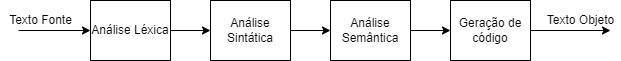
\includegraphics[scale=0.75]{Imagens/traducao.png}
\caption{Processo de tradução}
% \ref{sec:figs}
\label{fig:processo_traducao}
\end{figure}

%  blocos/fases/, fases e 
Os compiladores são estruturados em fases. Os modelos de organização dessas fases mais conhecidos são: análise-síntese e \textit{front-end} \textit{back-end}. O primeiro modelo é dividido, como o próprio nome apresenta, na etapa de análise, abrangendo todas as fases com esse nome além da geração da tabela de símbolos e rotina de tratamento de erros, e na etapa de síntese, referente às produções realizadas pelo mesmo: geração de código intermediário, otimizador desse código e gerador de código final. Esta organização é apresentada na Figura \ref{fig:modelo_analise_sintese}.

% \begin{figure}[ht]
%     \centering
%     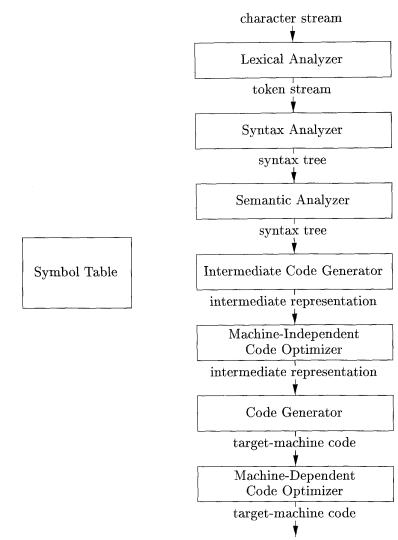
\includegraphics[scale=0.7]{Imagens/diagrama_fases_compilador_livro.png}
%     \caption{Fases de um compilador \cite{book_compilers}}
%     \label{fig:fases_compilador}
% \end{figure}

\begin{figure}[ht]
    \centering
    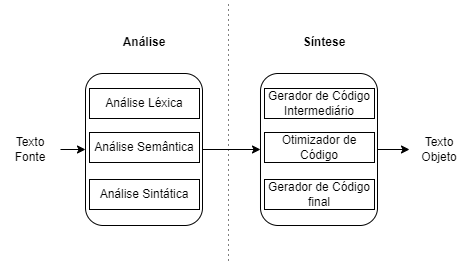
\includegraphics[scale=0.6]{Imagens/modelos_organizacionais_compiladores-analise_sintese.drawio.png}
    \caption{Fluxograma esquemático da organização análise-síntese dos compiladores}
    \label{fig:modelo_analise_sintese}
\end{figure}



Já em relação ao modelo \textit{front-end}/\textit{back-end}, além das etapas de análise, o \textit{front-end} também possui a etapa de geração do código intermediário, enquanto a segunda etapa volta-se apenas para a otimização deste e geração do texto objeto. Essa organização é visualizada na Figura \ref{fig:modelo_front_back}.
É importante ressaltar que alguns compiladores possuem uma fase de otimização da máquina-independente entre o \textit{front-end} e \textit{back-end} \cite{book_compilers}.

\begin{figure}[ht]
    \centering
    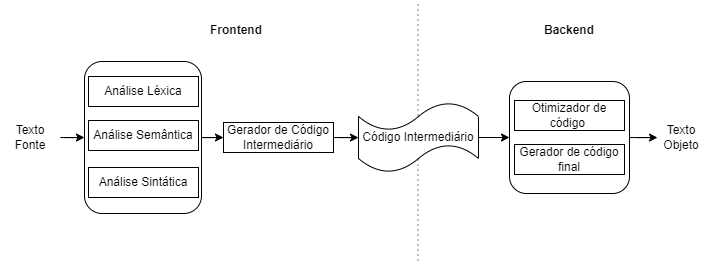
\includegraphics[scale=0.5]{Imagens/modelos_organizacionais_compiladores_front_back.drawio.png}
    \caption{Fluxograma esquemático da organização \textit{front-end} \textit{back-end} dos compiladores}
    \label{fig:modelo_front_back}
\end{figure}

\subsection{Processamento de Linguagem Natural}
Processamento de linguagem natural, também chamado entendimento de linguagem natural, é considerado uma ramificação da inteligência artificial, a qual utiliza as ferramentas computacionais para analisar, determinar similaridade semântica entre as linguagens e traduzi-las de forma automatizada \cite{NLP_book} \cite{NLP_ml_and_protein}. Esse estudo é aplicado tanto no texto escrito, quanto nos discursos, podendo ser classificado como: \textit{natural language processing}, para leitor/ouvinte, e \textit{generation}, escritor/orador.

O estudo sobre NLP surgiu a partir de década de 1940, tendo o \textit{Machine Translator} como o primeiro computador baseado em uma aplicação relacionada à linguagem natural, utilizando de tradução computacional para quebrar códigos inimigos durante a Segunda Guerra Mundial, e inspirando muitos outros projetos. Esse episódio provocou o uso da criptografia e da teoria da informação para a tradução de idiomas, onde os primeiros sistemas utilizavam apenas dicionários sem considerar ambiguidade lexical, o que provocou a conclusão de que a tradução era mais complicado do que havia sido previamente pensado e necessitando de uma teoria de linguagem mais adequada \cite{liddy2001natural}.

Com a publicação “\textit{Syntactic Structures}”, de Noam Chomsky, o conceito de gramáticas generativas mudou o mundo, já que se propôs a construção do que poderia gerar todas as sentenças de ma língua, tornando a sintaxe como centro da linguística e desafiando a explicação de como o significado de uma frase surge a partir dos significados de palavras individuais \cite{NLP_book}. Isso provocou o crescimento do processamento de linguagem natural.

Por muitos anos as seguintes suposições foram a base dessa temática: o estado que a gramática inglesa pode ser definida e utilizada para análise de qualquer parte da linguagem; e que o conhecimento contextual pode ser armazenado e utilizado para elucidação automática do significado \cite{NLP_book}. Entretanto, com o passar do tempo, o NLP original motivou recorrer a abordagens quantitativas no processamento automatizado de linguagem. 

Hoje, o processamento de linguagem natural possui uma arquitetura de \textit{pipeline}, que consiste na paralelização da execução das instruções de modo a maximizar a vazão das instruções realizadas. A Figura \ref{fig:pipeline_NLP} demonstra essa arquitetura. 

\begin{figure}[ht]
\centering
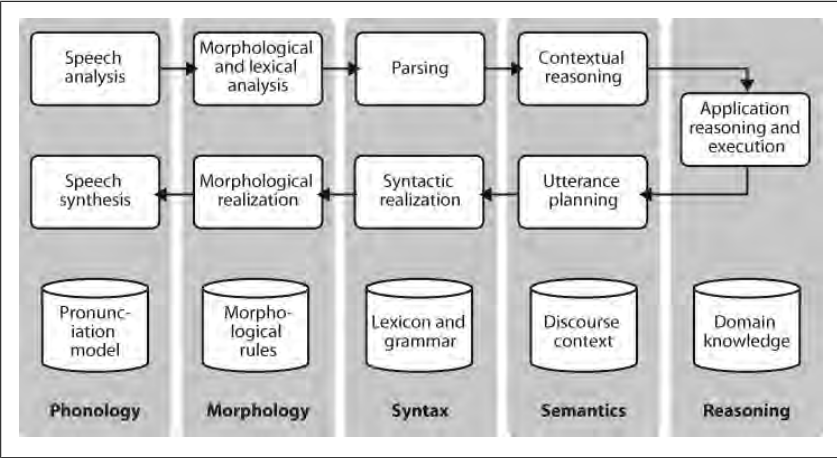
\includegraphics[scale=0.65]{Imagens/pipeline_architecture_nlp_system.png}
\caption{\textit{Pipeline} para um sistema de diálogo \cite{bird2009natural}}
\label{fig:pipeline_NLP}
\end{figure}

Como exemplificado na Figura \ref{fig:pipeline_NLP}, o NLP subdivide-se nos denominados “níveis de linguagem”, os quais são: fonologia, relacionada à interpretação dos sons do discurso dentro e através das palavras; morfologia, referida à estrutura individual das palavras; léxico, voltada para o vocábulo apresentado; sintaxe, remetida para a estrutura das sentenças e as suas regras de construção; semântica, relacionada à determinação do significado da sentença elaborada; discurso, este concentra-se nas propriedades do texto todo que transmitem sentido ao efetuar conexões entre frases e componentes; e pragmática, a qual tem o uso da linguagem em situações e utiliza contextos além do conteúdo do texto, requerendo muito conhecimento de mundo \cite{NLP_book} \cite{liddy2001natural}. 

Esses níveis podem não ser aplicados em todo sistema NLP, tendo em vista seu objetivo. Um exemplo disso é uma aplicação que não necessite de interpretação de alto nível, ou aplicações de baixo nível, no caso de unidades menores de análise (palavras ou sentenças) \cite{liddy2001natural}.

Somado a isso, a estrutura de sintaxe pode ser criada através do uso de gramáticas que especificam as regras da linguagem. Uma categoria de gramática comum usada no processamento natural de linguagem são as gramáticas livres de contexto (CFGs) \cite{NLP_book}. Entretanto, essa adoção provoca algumas limitações, como senso de ambiguidade, visto que as palavras podem assumir diferentes significados de acordo ao contexto tratado, denominado polissemia por \cite{NLP_book}.


\subsection{Sistemas de Auxílio a Decisão Clínica} %Maria

Um sistema de auxílio a decisão clínica objetiva orientar um profissional de saúde, ou um paciente, aconselhando o tratamento adequado, pontos de atenção, como alergias ou contraindicações médicas e, até mesmo, diagnóstico \cite{lichtenstein2011sistemas}. Esses sistemas podem acessar múltiplas bases de conhecimento, sendo capazes  de lidar com um grande volume de dados, e com a aplicação de inteligência artificial, os SADC conseguem trabalhar colaborativamente com os profissionais de saúde \cite{artigo_base}. Contudo, um dos principais desafios enfrentados é a integração com bases de dados grandes e heterogêneas \cite{CDSS_critical_care}.

A estrutura dos CDSSs pode ser concebida como um arco neural, em que seus receptores residem e são ativados pelos dados do paciente, seu centro de integração contém as regras de decisão e a base de conhecimentos; e seus efetores são as avaliações e recomendações específicas do paciente \cite{CDSS_critical_care}.

% história
Em 1959, Ledley e Lusted descreveram a lógica e probabilidade nas tomadas de decisões médicas. As contribuições de Sherppard e Kouchoukos no uso de medidas e regras automatizadas como potencial substituto para o julgamento no espaço de cuidado crítico mais avançado no campo. Mas, só após cerca de 20 anos chegou-se a um consenso sobre a definição de SADCs. Historicamente, esses sistemas foram divididos em: de suporte orientado pelo conhecimento, provendo a habilidade de inferir diagnósticos corretos; e por dados, mais utilizado nos casos que requerem tomadas de decisões médicas e cirúrgicas \cite{CDSS_critical_care}.

Esses sistemas visam uma colaboração  humano-IA capaz de favorecer o aprendizado mútuo, visto que o sistema fornece novas opiniões e correlações entre dados, enquanto os profissionais interagem com o SADC corrigindo eventuais erros de análise, e consequentemente, enriquecendo seu treinamento. Assim, é fundamental que os SADCs sejam dinamicamente modificáveis, pois os profissionais devem ter a palavra final nos diagnósticos e recomendações, além de serem eficientes apresentando os resultados em tempo hábil e exibindo apenas alertas relevantes\cite{artigo_base}.

Os SADCs precisam responder com um alto nível de qualidade e exatidão, considerando a sensibilidade dos dados analisados e sua aplicação. Logo, são utilizadas diretrizes, que se referem ao domínio médico dos processos e planos que justificam as ações dos profissionais. Segundo Field e Lohr, são definidas como “declarações desenvolvidas sistematicamente de forma a assistir às decisões de profissionais de saúde e pacientes sob determinados cuidados na saúde, para uma dada específica circunstância” \cite{lichtenstein2011sistemas}.


Para facilitar a análise de diretrizes clínicas, equipes de pesquisadores trabalharam na codificação das diretrizes dissertativas em diretrizes digitais, que podem ser implementadas via SADC, o que resultou em metas de uso mais eficientes \cite{lichtenstein2011sistemas}. 


Os sistemas de apoio à decisão clínica fornecem aconselhamento para casos específicos a partir dos dados do paciente e do conhecimento presente nas suas bases, considerando a interação constante com os profissionais de saúde, como representado na Figura \ref{fig:esquema_SADC}.

\begin{figure}[ht]
\centering
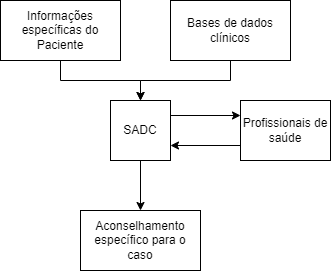
\includegraphics[scale=0.6]{Imagens/SADC.png}
\caption{Funcionamento de um SADC}
\label{fig:esquema_SADC}
\end{figure}

% NLP X COMPILADORES X SADC: Relação entre NLP e compiladores. Relação entre os 3
% resultados
\section{Processamento de linguagem natural e SADCs}

%destacar relação de colaboração humano-ia
A utilização de SADCs envolve um trabalho conjunto entre a equipe médica e o sistema de inteligência artificial, por um compartilhamento bilateral de informações e construção iterativa do conhecimento \cite{artigo_base}. Dessa forma, faz-se necessário o estabelecimento de diálogo entre os profissionais de saúde e o sistema, que ocorre por meio da linguagem natural, como o acompanhamento do prontuário eletrônico dos pacientes \cite{lichtenstein2011sistemas}.

Considerando o volume crescente de dados clínicos, registrados pelos profissionais da saúde, e a necessidade de sua recuperação e análise, evidencia-se a importância de um resgate eficiente dessas informações \cite{prontuario_PLN}. Contudo, apesar da utilização de registros eletrônicos apresentar benefícios como facilidade de armazenamento e filtragem do conteúdo, os textos ainda são inseridos livremente em uma narrativa clínica que possui um nível de detalhamento variável, dificultando a recuperação da informação \cite{prontuario_PLN}.

Considerando a aplicação do processamento de linguagem natural em diversas áreas, no que tange os sistemas de apoio à decisão clínica, o processo de extração de informações é reconhecido como uma área especializada em NLP \cite{WANG201834}. Essa etapa se refere à extração automática de conceitos, entidades e eventos, como também suas relações e atributos de texto livre. Essas extrações podem ser utilizadas para uma gama de aplicações, como perguntas-respostas, visualização e mineração de dados \cite{liddy2001natural}.

A maioria dos sistemas de extração de informações são baseados em sistemas que consistem em padrões os quais definem restrições léxicas, sintáticas e semânticas. Dessa forma, no domínio clínico, os sistemas NLPs são usados para identificar, por exemplo, síndromes clínicas, lista de problemas, documentação de enfermagem e educação médica \cite{WANG201834}. Alguns autores buscaram a aplicação desses sistemas em áreas específicas na medicina, como a identificação de casos de câncer através da radiologia ou por colonoscopia, como é apresentado na pesquisa realizada por \cite{algorithm_cdss}. 

Segundo \cite{what_can_nlp_cdss}, para que um sistema de apoio à tomada de decisões clínicas dependa do processamento de linguagem natural, deve ser confiável, de alta-qualidade de desempenho e modular, flexível e possua rápidos sistemas. A integração desses sistemas pode ser ativa ou passiva em que, a primeira alavanca informações existentes e envia informações específicas do paciente para usuários, já a segunda, necessita da entrada do usuário para gerar os resultados. Para os dois tipos, o processamento pode originar-se de fontes textuais, como gravações clínicas, literatura biomédica, páginas \textit{web} e notas de suicídio.

O processamento de linguagem natural voltado para o contexto dos sistemas de apoio à tomada de decisões clínicas, pode ser dividido em \cite{what_can_nlp_cdss}:

\begin{itemize}
    \item \textbf{Pré-processamento textual}: voltada para a atribuição de \textit{tokens} (simbolização), com a identificação dos termos e etiquetagem da parte da fala e análise sintática. Uma aplicação é a expansão de abreviaturas e correções ortográficas, buscando evitar problemas de desambiguação do sentido. Erros no nível de fala, podem propagar-se atingindo a análise sintática e, assim, a semântica tanto da narrativa clínicas, quanto da literatura biomédica e, consequentemente, no entendimento do próprio texto.
    
    \item \textbf{Reconhecimento de entidade nomeada (NER)}: identifica os limites do nome no texto e entende seu significado através do mapeamento da entidade para um identificador de conceito. Para isso, necessita-se de um dicionário baseado nessa entidade o qual provenha uma lista de nomes para uma categoria de entidade dada, um exemplo de método de sucesso é o aprendizado supervisionado para NER biomédicos.
    
    \item \textbf{Extração de contexto}: uma das funções chaves é a extração do contexto de um evento ou entidade, a qual pode ser através de um algoritmo a exemplo do \textit{ConText} (citar).
    
    \item \textbf{Associação e extração de relações}: através da identificação e extração dos relacionamentos entre as entidades identificadas e os eventos. Similar ao NER, podendo decompor a relação tirada em relação detectada e determinação do seu tipo.

\end{itemize}

Um exemplo de sistema de NLP nos SADCs é o \textit{Medical Language Extraction and Encoding System} (MedLEE) é um sistema desenvolvido em 1994, primeiro projetado para relatórios da radiologia sendo estendido para outros domínios como sumários de descargas \cite{nlp_biomedicine_arquitecture}. Esse sistema é dividido no conhecimento base, o qual inclui conceitos médicos, e no processador de linguagem natural. A Figura \ref{fig:medLEE_arquitetura} demonstra a arquitetura do sistema.

\begin{figure}[ht]
    \centering
    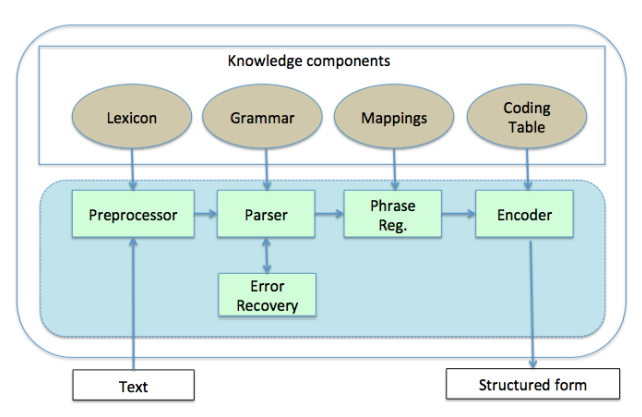
\includegraphics[scale=0.67]{Imagens/fluxograma_arquitetura_nlp_medLEE.png}
    \caption{Arquitetura do MedLEE \cite{nlp_biomedicine_arquitecture}}
    \label{fig:medLEE_arquitetura}
\end{figure}

% processamento de lingaugem natural como um caminho para essa colaboração

\section{Compiladores e Processamento de Linguagem Natural}

Uma  alternativa para possibilitar a comunicação entre o usuário e um sistema utilizando a linguagem natural é a utilização de um \textit{software} capaz de traduzir um texto fonte em uma linguagem natural para um texto objeto interpretável por uma \textit{framework} de programação \cite{compiler_natural_language}.

Como um dos desafios do desenvolvimento de SADCs é o gerenciamento de uma abundância de dados expressos em texto livre, a tradução desse conteúdo para um texto intermediário em estrutura de \textit{queries} facilitaria o gerenciamento da informação. Esse processo de tradução pode ser realizado com o auxílio de um s\textit{oftware } que funcionaria  como um compilador de linguagem natural, capaz de converter um texto fonte em linguagem natural para um texto objeto intermediário composto por estruturas semânticas mais simples \cite{compiler_on-line_data}.

Compiladores possibilitam a conversão de um código escrito em linguagens de programação de alto nível para um texto em uma linguagem de baixo nível. Assim, seguindo a estrutura de funcionamento de um compilador, é possível realizar a tradução de um texto em linguagem natural para um texto interpretável por um sistema de auxílio a decisão clínica \cite{compiler_code_conversion}.

É possível verificar a correlação entre a técnica de desenvolvimento de compiladores com o algoritmo desenvolvido no trabalho de \cite{algorithm_cdss}, capaz de realizar a análise gradual de relatórios de colonoscopia e patologia. Inicialmente, realizou-se a \textit{tokenização} dos parágrafos em sentenças, que em seguida, foram divididas em palavras numeradas, possibilitando a elaboração de uma tabela equivalente à tabela de símbolos construída no processo da compilação. Essa etapa abordada corresponde à análise léxica realizada por um compilador. 

Outro exemplo é o HiTEx (\textit{Health Information Text Extraction}, o qual realiza a montagem de narrativas clínicas dos pacientes através de \textit{pipelines} para a extração de conclusões específicas. Essa arquitetura é formada aplicando sequencialmente uma divisor de seção, filtro de seção, divisor de frases, \textit{tokenizador} de sentenças, \textit{POStagger}, buscador de substantivos, conceitos de mapeamento em UML (\textit{Unified Modeling Language}) e localizador de negação \cite{what_can_nlp_cdss}. Nesse exemplo, pode-se fazer a analogia não só aos compiladores em si, mas também aos pré-processadores em relação à aplicação dos filtros, já quanto a de divisor de seções e frases, percebe-se a semelhança das atividades realizadas pelo analisador léxico, e mais uma vez, a atribuição de símbolos da análise sintática na atribuição de \textit{tokens} nas sentenças.

A aplicação dos CDSSs utilizando NLPs nos eventos de monitoramento clínico é um dos exemplos trazidos por \cite{what_can_nlp_cdss}. Ela é composta pelos seguintes passos: identificação do evento alvo (\textit{target}); seleção do repositório de dados clínicos; processamento de linguagem natural para representação de narrativa clínica formal; geração de \textit{query} para detecção do evento e classificação; verificação da acurácia de detecção e classificação; análise de erros; melhoria iterativa nos 1º, 3º e 4º passos baseado nos últimos. Nessas etapas, podemos visualizar a aplicação direta da rotina de tratamento de erros nos últimos 3 passos, a geração do código otimizado também na última parte, mais especificamente, em sua aplicação na 3ª fase, a geração do código intermediário na utilização do NLP.
 


Dessa forma, nota-se que a aplicação direta da teoria de compiladores pode auxiliar no desenvolvimento de sistemas de processamento de linguagem natural focados na análise de relatórios clínicos. O processo de tradução do texto fonte em linguagem natural (fonte) em um texto objeto composto por estruturas sintáticas mais simples pode facilitar a coleta de dados dos sistemas de análise clínicas e, consequentemente, o armazenamento, busca e interpretação das informações. 

% fazer a comparação - relação direta (cada etapa da construção de sistemas NLPs com a compilação)

\section{Conclusão}

Neste artigo, apresentamos a correlação entre o desenvolvimento de sistemas de apoio a decisão clínica, as técnicas de construção de compiladores e utilização do processamento de linguagem natural. Assim, é possível compreender um dos principais desafios da comunicação entre os profissionais da área médica e os SADCs: a tradução de um texto fonte em linguagem natural para um texto objeto em uma linguagem interpretável pelo sistema.

Ao analisar o processo de tradução executado pelos compiladores foi possível estabelecer um paralelo entre esses \textit{softwares} e a técnica de processamento de linguagem natural, pois possuem o objetivo em comum de automatizar o processo de tradução. Entre as semelhanças identificadas encontram-se: a realização das análises léxica, sintática, semântica, rotinas de tratamento de erros, geradores de códigos intermediários e final, além da geração e administração da tabela de símbolos.
Assim, a aplicação da teoria de compiladores em soluções voltadas para NLP mostra-se uma alternativa para viabilizar a tradução de relatórios médicos em diversas especialidades e prontuários, favorecendo a interação entre os profissionais e os sistemas.

%digitar conclusão, máximo dois parágrafos

\bibliographystyle{sbc}
\bibliography{sbc-template}

\end{document}
